
\documentclass{article}
%\documentclass[10pt,letterpaper]{article}
%\usepackage[top=0.85in,left=2.75in,footskip=0.75in]{geometry}

% amsmath and amssymb packages, useful for mathematical formulas and symbols
%\usepackage{amsmath,amssymb}

% Use adjustwidth environment to exceed column width (see example table in text)
%\usepackage{changepage}

% Use Unicode characters when possible
%\usepackage[utf8x]{inputenc}

% textcomp package and marvosym package for additional characters
%\usepackage{textcomp,marvosym}

\usepackage{graphicx}
\usepackage[english]{babel}
\usepackage{amsmath,amsthm}
\usepackage{amsfonts}

\begin{document}
\title{Social Force in Pedestrian Crowd}
\author{Peng Wang}%

%\address{}%
%\email{}%

%\thanks{}%
%\subjclass{}%
\maketitle

% ----------------------------------------------------------------
\begin{abstract}
This paper provides a new perspective to understand existing controversy on the social force model.  These issues include that the social force disobeys Newton 3rd Law, oscillation phenomenon when one agent is approaching another as well as some questions on the faster-is-slower effect.  From the perspective of physics these problems seems difficult to explain.  This paper provides a new perspective to understand these issues.  We introduce a new concept of desired interpersonal distance to explain how the social force is generated from conscious mind of human.  Although the social force disobeys Newton 3rd Law, the whole model is exactly within the Newton Laws to characterize pedestrian motion.  The oscillation phenomenon may exist in non-physics entity (i.e., desired velocity and desired interpersonal distance) rather than physics entity (i.e., actual velocity and actual distance), and such oscillation is mitigated by treating non-physics entity as variable rather than constant.  Very interestingly, the desired velocity represents the motivation level of pedestrian motion, and the faster-is-slower effect is thus explained by Yerkes–Dodson law, explaining how motivation level could improve or impair human performances in a collective sense.  This inverted-U effect is further studied with a falling-down model and the numerical testing is exhibited by using FDS+Evac.
\end{abstract}


\section{About Social Force Model}

The social-force model presents psychological forces that drive pedestrians to move as well as keep a proper distance with others.  In this model an individual's motion is motivated by a self-driving force fiself and resistances come from surrounding individuals and facilities (e.g., walls).  Especially, the model describes the social-psychological tendency of two individuals to keep proper interpersonal distance (as called the social-force) in collective motion, and if people have physical contact with each other, physical forces are also taken into account.  Let $\mathbf{f}_{ij}$ denote the interaction from individual $j$ to individual $i$, and $\mathbf{f}_{iw}$ denote the force from walls or other facilities to individual $i$.  The change of the instantaneous velocity $\mathbf{v}_i(t)$ of individual $i$ is given by the Newton Second Law:

%
\begin{equation}\label{Eq_Newton2ndLaw}
    m_i \frac{d \mathbf{v}_i(t)}{dt} = \mathbf{f}_i^{drv} +
	\sum_{j \ne i} \left( \mathbf{f}_{ij}^{soc} + \mathbf{f}_{ij}^{phy} \right) +
	\sum_{w} \left( \mathbf{f}^{soc}_{iw} + \mathbf{f}^{phy}_{iw} \right) ~,
\end{equation}
%

where $\mathrm{m}_i$ is the mass of individual $i$. Furthermore, the self-driving force $\mathbf{f}_i^{drv}$ is specified by

%
\begin{equation}\label{Eq_self_driving_force}
  \mathbf{f}_i^{drv} = \frac{m_i}{\tau_i} \left( \mathbf{v}_i^0 -
    \mathbf{v}_i\right) ~,
\end{equation}
%

This force describes an individual tries to move with a desired velocity $\mathbf{v}_i^0(t)$ and expects to adapt the actual velocity $\mathbf{v}_i(t)$ to the desired velocity $\mathbf{v}_i^0(t)$ within a certain time interval $\tau_i$. In particular, the desired velocity $\mathbf{v}_i^0(t)$ is the target velocity existing in one's mind while the actual velocity $\mathbf{v}_i(t)$ characterizes the physical speed and direction being achieved in the reality.  The gap of $\mathbf{v}_i^0(t)$ and $\mathbf{v}_i(t)$ implies the difference between the human subjective wish and realistic situation, and it is scaled by a time parameter $\tau_i$ to generate the self-driving force.  This force motivates one to either accelerate or decelerate, making the realistic velocity $\mathbf{v}_i(t)$ approaching towards the desired velocity $\mathbf{v}_i^0(t)$.  This mathematical description of the self-driving force could be dated back to the Payne-Whitham traffic flow model (Payne, 1971; Whitham, 1974).  Sometimes $\mathbf{v}_i^0(t)$ is rewritten as $\mathbf{v}_i^0(t) = v_i^0(t)\mathbf{e}_i^0(t)$, where $v_i^0(t)$ is the desired moving speed and $\mathbf{e}_i^0(t)$ is the desired moving direction.  In a similar manner, we also have $\mathbf{v}_i(t) = v_i(t)\mathbf{e}_i(t)$ where $v_i(t)$ and $\mathbf{e}_i(t)$ represent the physical moving speed and direction, respectively.

%The interaction force of pedestrians consists of the social-force f_{ij}^{soc} and physical %interaction f_{ij}^{phy} . i.e., .	 The social-force f_{ij}^{soc} characterizes the %social-psychological tendency of two pedestrians to stay away from each other, and it is %given by

%
\begin{equation}\label{Eq_socialforce}
 \mathbf{f}_{ij}^{soc} = A_i e^{-(d_{ij}-r_{ij})/B_i }
 \left ( \lambda_i + (1-\lambda_i) \frac{1 + \cos \varphi_{ij}}{2}
 \right )  \mathbf{n}_{ij} ~,
\end{equation}
%

\noindent where $A_i$ and $B_i$ are positive constants, which affect the strength and effective range about how two pedestrians are repulsive to each other.  The distance of pedestrians $i$ and $j$ is denoted by $d_{ij}$ and the sum of their radii is given by $r_{ij}$ .  $\mathbf{n}_{ij}$ is the normalized vector which points from pedestrian $j$ to $i$.  The geometric features of two pedestrians are illustrated in Figure 1.  In practical simulation, an anisotropic formula of the social-force is widely applied where Equation ~(\ref{Eq_socialforce}) is scaled by a function of $λ_i$.  The angle $\phi_{ij}$  is the angle between the direction of the motion of pedestrian $i$ and the direction to pedestrian $j$, which is exerting the repulsive force on pedestrian $i$. If $λ_i = 1$, the social force is symmetric and $0 < λ_i < 1$ implies that the force is larger in front of a pedestrian than behind.  This anisotropic formula assumes that pedestrians move forward, not backward, and thus we can differ the front side from the backside of pedestrians based on their movement.  Although the anisotropic formula is widely used in pedestrian modeling, it also brings a controversial issue that the anisotropic formula of social force disobeys Newton's 3rd law.

%
\begin{figure}[tb]
  \centerline{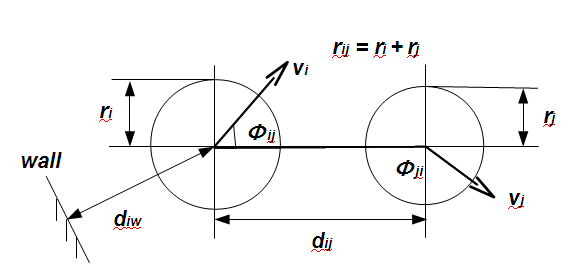
\includegraphics[clip=true, width=30mm, scale=0.3]{FIGURES/twoAgents.png}}
  \caption{A Schematic View of Two Pedestrians (Equation ~(\ref{Eq_socialforce})):
The distance of pedestrians $i$ and $j$ is denoted by $d_{ij}$ and the sum of their radii is given by $r_{ij}$. The distance to the wall is denoted by $d_{iw}$.}\label{Fig_twoAgents}
\end{figure}
%

The physical interaction $f_{ij}^{phy}$ describes the physical interaction when pedestrians have body contact, and it is composed by an elastic force that counteracts body compression and a sliding friction force that impedes relative tangential motion of two pedestrians.  Both of them are valid only when $r_{ij} > d_{ij}$.  In Helbing, Farkas and Vicsek, 2000 the interaction force is repulsive.  The model may also include an attraction force in its original version (Helbing and Molnar, 1995, Korhonen, 2015).  The interaction of a pedestrian with obstacles like walls is denoted by \$mathbf{f}_{iw}$ and is treated analogously, i.e., $\mathbf{f}_{iw} = \mathbf{f}_{iw}^{soc} + \mathbf{f}_{iw}^{phy}$.  Here $\mathbf{f}_{iw}^{soc}$  is also an exponential term and $\mathbf{f}_{iw}^{phy}$ is the physical interaction when pedestrians touch the wall physically.  

%
\begin{figure}[tb]
  \centerline{\includegraphics[clip=true, width=30mm, scale=0.3]{FIGURES/helbingFramework.png}}
  \caption{From Particle Dynamics to Crowd Simulation: The Framework of Many-particle Simulation in Helbing, Farkas, and Vicsek, 2000}\label{Fig_helbingFramework}
\end{figure}
%

	
\section{Social Force and Newton Third Law}

This section provides a psychological perspective to reinterpret the social-force, and the concepts of interpersonal distance, proxemics and stress are critically involved.  Very importantly we introduce a new concept of desired distance in the social force, which is the counterpart of the desired velocity in the self-driving force.  With this new concepts we further discuss whether the model is consistent with Newton 3rd Law.


\noindent \textbf{ A. Interpersonal Space and Social-Force}

The concept of social force may originate from a concept by Lewin (Lewin, 1951), where social fields or social forces were first introduced to guide behavioral changes of people.  In soci-psychology, such social fields or forces are representations of certain social norms that regulate people's behavior when one individual interacts with others.  In a spatial sense such social norms refers to how people use their interpersonal distance, and it refers to proxemics in psychological theories.

Interpersonal distance refers to a theory of how people use their personal space to interact with surrounding people.  In Hall, 1963 the theory was named by proxemics, and it was defined as "the interrelated observations and theories of man's use of space as a specialized elaboration of culture."  Proxemics suggests that we surround ourselves with a "bubble" of personal space, which protects us from too much arousal and helps us keep comfortable when we interact with others.  Psychologically, proximal distance origins from basic human instincts that we define a personal space to get a sense of safety.  People normally feel stressed when their personal space is invaded by others.  There are four interpersonal distances mentioned in Hall, 1966: intimate (\l 0.46m), personal (0.46m to 1.2m), social (1.2m to 3.7m), and public (\g 3.7m), and each one represents a kind of social relationship between individuals.  Here we highlight two issues about proxemics as below.

\noindent (a)  The interpersonal distance is object-oriented. For example, we usually keep smaller distance to a friend than to a stranger, and such distance is an indication of familiarity.  As named by personal distance (0.46m to 1.2m) in proxemics, this range is widely observed as the distance to interact with our friends or family, and normal conversations take place easily at this range.

\noindent (b) The interpersonal distance reflects a kind of social norms.  For example, in a crowded train or elevators, although such physical proximity is psychologically disturbing and uncomfortable, it is accepted as a social norm of modern life.  Also, it is also known that the male and female commonly keep larger distance in public place in Muslim culture than other cultures.  In brief although proximal distance origins from basic human instincts, it is also widely redefined in different social norms.


Proxemics implies that when the interpersonal distance is smaller than the desired, people feel stressed.  Repulsion comes into being in this situation, and repulsion increases when the distance further decreases.  This theory justifies the assumption of repulsive social-force in Equation ~(\ref{Eq_socialforce}).  However, such repulsion does not depend on physical size of two people (i.e., $r_{ij}$), but the social relationship, occasions and social norms.  Similar to self-driving force we suggest that it is proper to add a subjective concept of desired distance $d_{ij}^0$ in the social force, and it replaces $r_{ij}$ in Equation ~(\ref{Eq_socialforce}).  Here $d_{ij}^0$ is the target distance that individual i expects to keep with individual $j$.  This distance describes the social relationship of individual $i$ and $j$ .  Based on the exponential form in Equation ~(\ref{Eq_socialforce}), the social force is rewritten as

%
\begin{equation}\label{Eq_newsocialforce}
 \mathbf{f}_{ij}^{soc} = A_i \left ( \lambda_i + (1-\lambda_i) \frac{1 + \cos \varphi_{ij}}{2} \right ) exp \left( -(d_{ij}-d_{ij}^0)/B_i \right) \mathbf{n}_{ij} ~,
\end{equation}
%

Similar to desired velocity $mathbf{v}_i^0$, the desired distance $d_{ij}^0$ is the target distance in one's mind, specifying the distance that one expects to adapt oneself with others.  The physical distance $d_{ij}$ is the distance achieved in the reality. The gap of $d_{ij}^0$ and $d_{ij}$ implies the difference between the subjective wish in one's mind and objective feature in reality. Here $A_i$ and $B_i$ are parameters as introduced before, and $mathbf{n}_{ij}$ is the normalized vector which points from pedestrian $j$ to $i$. In a similar manner, an anisotropic formula of social-force is also modified in Equation ~(\ref{Eq_newsocialforce}). The social force also functions in a feedback manner to make the realistic distance dij approaching towards the desired distance $d_{ij}^0$. A difference is that $v_i^0$ and $v_i$ are vectors while $d_{ij}^0$ and $d_{ij}$ are scalars.

A major difference between the concepts of $r_{ij}$ and $d_{ij}^0$ is that $r_{ij}$ is a physics-based concept and it is normally a constant. In contrast $d_{ij}^0$ is neither a constant nor a physics entity. In brief, $d_{ij}^0$ describes people's opinion, and it may vary as the opinion changes. For example, when crowd wait at a narrow entrance, people accept smaller interpersonal distance, and thus $d_{ij}^0$ is tuned to be a smaller value so that their repulsion is reduced. Reducing repulsion in certain conditions has been applied in
crowd simulation such as FDS+Evac (Korhonen, 2017). On the other side the coding framework of social-force model is not directly affected when $r_{ij}$ is replace by $d_{ij}^0$ in computer programs When realizing the model in computer programs, $r_{ij}$ and $d_{ij}^0$ are exactly at the same position, and we can simply transform $r_{ij}$ to $d_{ij}^0$ by using $d_{ij}^0 = r_{ij} c_{ij}$ such that the existing program is extended for the new force. Here $c_{ij}>1$ is a scale factor.

In a psychological sense $d_{ij}^0$ and $v_i^0$ are both subjective concepts which exist in people's mind, and they characterize how an individual intends to interact with others and environment.  As a result, the social-force given by Equation ~ (\ref{Eq_newsocialforce}) and the self-driving force are both subjective forces which are generated involving one's mental activities and opinions. In a physics sense the subjective forces are generated by the foot-ground friction, which exactly obey physics laws. The social force model thus exhibits a bridge between the physics laws and psychological principles regarding crowd motion.


\noindent \textbf{B. Social Force and Newton Third Law}

A common criticism about the social force model is that the anisotropic formula of social force disobeys Newton's 3rd law, and thus it becomes questionable in field of physics studies.  In addition, Equation ~(\ref{Eq_newsocialforce}) implies that $d_{ij}^0$ may be different from $d_{ji}^0$.  As a result, the social force between two individuals is not balanced, i.e.,  $d_{ij}^0 \neq d_{ji}^0$ and $f_{ij}^{soc} \neq f_{ji}^{soc}$.  Thus, Newton third law (actio = reactio) does not hold either for Equation ~(\ref{Eq_newsocialforce}) even if the anisotropic formula is not used.

An interesting question is why the social force itself does not obey Newton 3rd Law.  The important issue is that $d_{ij}^0$ exists in human mind, and it is not a physics entity.  In a psychological sense $d_{ij}^0$ is a subjective concept which exists in people's mind, and it characterizes how an individual intends to interact with others.  As a result, the self-driving force and social force are both entities in subjectiveness, and they are generated involving one's intention and opinion.  If the anisotropic formula is also used, it further takes human foresight effect into account, where each individual pedestrian is more influenced by others in front than things behind.  In other words, the anisotropic formula of social force also assumes human perception, and it is not typically a physics concept either, but a subjective concept involving human perception and cognition.  Because the social force is not a physics concept, it does not follow Newton 3rd Law in its mathematical expression.

In real-world situation two individuals never have any physical interaction if they do not touch each other physically.  If a pedestrian want to keep a certain distance to anyone, he or she do not need to push or pull anyone, but move with their feet to adjust the distance.  In other words, people normally use foot-floor friction to realize the "social force."  So the foot-floor friction is a physics concept, and it is consistent with Newton 3rd Law for interaction between foot and floor.  The social force is not a physics concept, and it is just a part of foot-floor friction.

Currently the social force model is widely applied to movement of particles or living bodies.  If the social force model is used for nonliving things such as particles which interacts directly without other medium involved, the model disobeys Newton 3rd Law.  If the model is applied to pedestrian motion, such motion is realized by the interaction of pedestrian and the ground, and the social force is actually a part of foot-ground friction.  In general the social-force model is applicable to movement of any creature like human, bird or fish, and the media for their interaction could be ground, air or water.  The model is thus useful to characterize movement of any living forms with conscious mind.  When the ground is taken into account for human, the social force and self-driving force actually fit into Newton Laws, and Newton 3rd law is exactly valid at the physical level where the social force is viewed as a part of foot-ground friction.  The details of the above discussion is listed in the following table.

%
%Table
%
%
\begin{table}[b!]
\begin{center}
\caption{Unimpeded walking velocities and body dimensions in FDS+Evac.
   The offset of shoulder circles is given by $d_s = R_d - R_s$, for the
   definition of the other body size variables, $R_d$, $R_t$, $R_s$,
   see Fig.~\protect\ref{Fig_HumanBody}.  The body sizes and walking
   velocities of the agents are personalised by using them from uniform
   distributions, whose rages are also given.}\label{Table_DefaultHumans}
\vspace{12pt}
\begin{tabular}{l c c c c c}\hline\hline
Body type & $R_d$& $R_t/R_d$ & $R_s/R_d$  & $d_s/R_d$ & Speed \\
          & (m)  & (-)   &  (-)    & (-)    & (m/s) \\ \hline
Adult     & 0.255$\pm$0.035 & 0.5882 & 0.3725 & 0.6275 &
          1.25$\pm$0.30 \\  % +- 0.07m 0.30m/s
Male      & 0.270$\pm$0.020 & 0.5926 & 0.3704 & 0.6296 &
          1.35$\pm$0.20 \\  % +- 0.04m 0.20m/s
Female    & 0.240$\pm$0.020 & 0.5833 & 0.3750 & 0.6250 &
          1.15$\pm$0.20 \\  % +- 0.04m 0.20m/s
Child     & 0.210$\pm$0.015 & 0.5714 & 0.3333 & 0.6667 &
          0.90$\pm$0.30 \\  % +- 0.03m 0.30m/s
Elderly   & 0.250$\pm$0.020 & 0.6000 & 0.3600 & 0.6400 &
          0.80$\pm$0.30 \\ \hline\hline  % +- 0.04m 0.30m/s
\end{tabular}
\end{center}
\end{table}
%


As shown in Table 1 foot-floor friction is the physics-based force that drive pedestrians to move, and we can consciously control this friction to decide where and how fast we move.  In social force model such foot-floor friction consists of self-driving force, social force and so forth.  In sum the social force is a kind of interaction involving one's consciousness.  It is not typically a physics concept.  The social force characterizes whether an individual “desires” to be close or far away from others, and thus it inspires us to replace the individual radius by “desired interpersonal distance” to highlight this psychological effect.   As a pedestrian realizes this force in the physical world, the force is part of the foot-floor friction, which exactly obey Newton's laws between the human and the ground.  In other words Newton 3rd law still stands in pedestrian modeling where the social force is viewed as a part of foot-ground friction.  In a word the social-force model critically exhibits a bridge between the physics laws and psychological principles regarding crowd motion, and we consider this as a major contribution of the social force model.

\section{Oscillating Walkers In Collective Motion}


\chapter*{Acknowledgements}
\addcontentsline{toc}{chapter}{Acknowledgements}

\noindent The authors are thankful to Dr.\ Peter Luh and Dr.\ Kerry Marsh for helpful comments on earlier work in University of Connecticut.   The authors are also grateful to Dr.\ Timo Korhonen for helpful discussion in simulation work of FDS+Evac.  The author appreciates the  research program funded by NSF Grant # CMMI-1000495 (NSF Program Name: Building Emergency Evacuation - Innovative Modeling and Optimization).

\clearpage

\newpage

\addcontentsline{toc}{chapter}{References}
\renewcommand{\bibname}{References}
\begin{thebibliography}{99}

%
\bibitem{SMV_UserGuide} Forney, G.P., ``Smokeview, A Tool for
  Visualizing Fire Dynamics Simulation Data, Volume I: User's Guide'',
  NIST Special Publication 1017-1 6th Edition, National Institute of
  Standards and Technology, Gaithersburg, MA, June 2016, 188~p.
%
\bibitem{SMV_TechGuide} Forney, G.P., ``Smokeview (Version 6.1.5) - A
  Tool for Visualizing Fire Dynamics Simulation Data, Volume II:
  Technical Reference Guide'', NIST Special Publication 1017-1,
  National Institute of Standards and Technology, Gaithersburg, MA,
  August 2013, 70~p.
%
\bibitem{SMV_VVGuide} Forney, G.P., ``Smokeview (Version 6.1.5) - A
  Tool for Visualizing Fire Dynamics Simulation Data, Volume III:
  Verification Guide'', NIST Special Publication 1017-3, National
  Institute of Standards and Technology, Gaithersburg, MA, November
  2013, 88~p.

%
\bibitem{Helbing95} Helbing, D., and Moln\'ar, P., ``Social force
  model for pedestrian dynamics'', \emph{Physical Review E} 51:
  4282--4286 (1995).
%
\bibitem{Helbing00} Helbing, D., Farkas, I., and Vicsek, T.,
  ``Simulating dynamical features of escape panic'', \emph{Nature}
  407: 487--490 (2000).
%
% Next is for book
\bibitem{Helbing02} Helbing, D., Farkas, I., Moln\'ar, P., and
  Vicsek,T., ``Simulating of Pedestrian Crowds in Normal and
  Evacuation Situations'', \emph{Pedestrian and Evacuation Dynamics},
  Schreckenberg, M. and Sharma, S.D. (eds.), Springer, Berlin, 2002,
  pp.~21--58.

%
\bibitem{Proulx1993} Proulx, G., ``A Stress Model for People Facing a
  Fire'', \emph{Journal of Environmental Psychology} 13: 137--147,
  1993.
%
%\bibitem{Fang03} Fang, Z., Lo, S.M.\ and Lu, J.A., ``On the
%  Relationship between Crowd Density and Movement Velocity'',
%  \emph{Fire Safety Journal} 38: 271--283, 2003.
%

\bibitem{IMO07} IMO, ``Guidelines for Evacuation Analyses for
  New and Existing Passenger Ships'', MSC/Circ.1238, International
  Maritime Organization, London, UK, 30 October 2007.

%\bibitem{Rinne10} Rinne, T., Tillander, K., and Grönberg, P., ``Data
%  Collection and Analysis of Evacuation Situations,'' VTT Research
%  Notes 2562, VTT Technical Research Centre of Finland , Espoo,
%  Finland, 2010 (http://www.vtt.fi/publications/index.jsp).
%

%\bibitem{Heliovaara12} Heli\"ovaara, S., Korhonen, T., Hostikka, S.,
%  and Ehtamo, H., ``Counterflow model for agent-based simulation of
%  crowd dynamics'',  \emph{Building and Environment} 48: 89--100, 2012.
%
\end{thebibliography}

\end{document} 